\chapter{Results}

By implementing a microarchitecture comprised of a program counter, register, control and ALU modules, and wiring these together to form a control-/datapath, we succeded in implementing a multi-cycle, MIPS-like processor.
Each component was tested with individual testbenches.
The system as a whole was tested using an end-to-end testbench, as well as by uploading the bitfile to an FPGA in the lab and verifying correctness using the \texttt{hostcomm} utility.
We succeded in implementing support for the instructions listed as requirements in the exercise description.

Our implementation has two stages, Instruction Fetch and Instruction Execute.
The fetch stage is done in one clock period, while the execute stage is done in either one or two periods, depending on the instruction.

\begin{figure}[h!]
    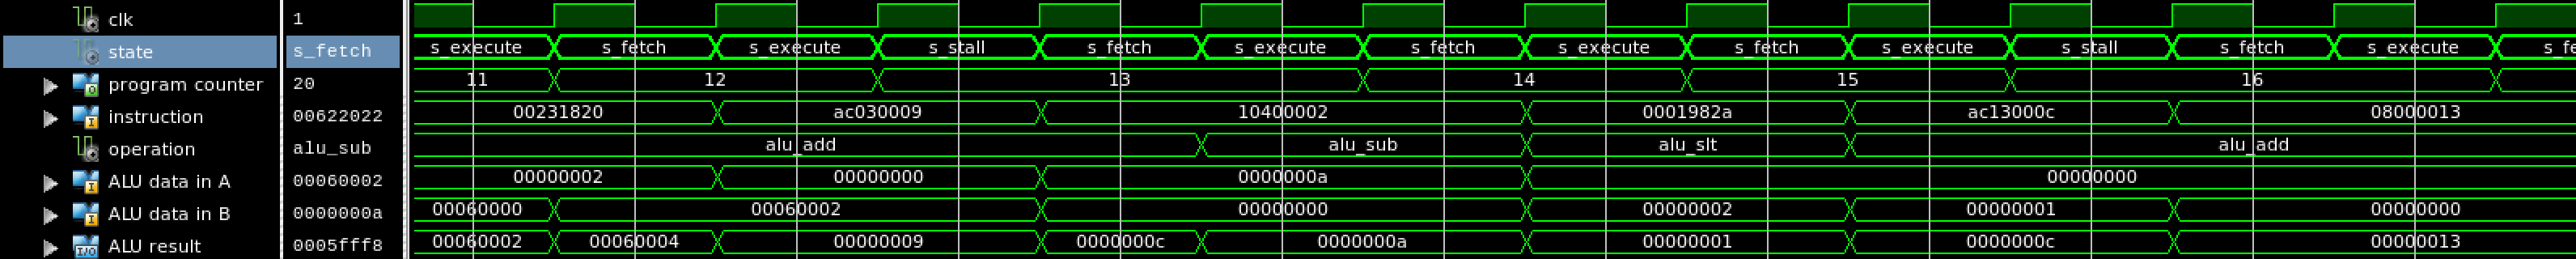
\includegraphics[width=\linewidth]{img/overview_sim.png}
    \caption{A screenshot from ISim, showing an overview of some important signals in our implementation.}
    \label{fig:waves}
\end{figure}

\begin{figure}[h!]
    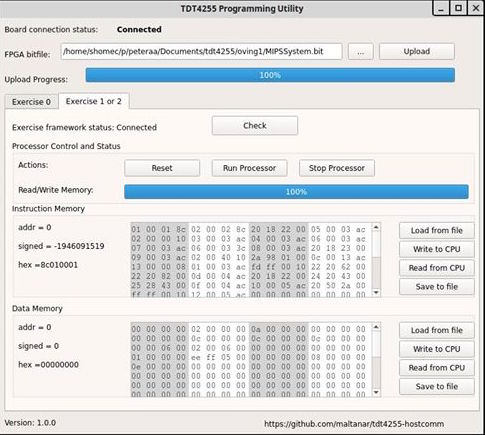
\includegraphics[width=\linewidth]{img/hostcomm.jpg}
    \caption{A screenshot of the hostcomm utility after allowing our processor to execute a simple program.}
    \label{fig:hostcomm}
\end{figure}

To explore how our design mapped out to an actual circuit we explored the generated RTL produced by xilinx in order to see how different the resulting RTL was from our ideal RTL.
Some interesting results include how for instance the synthesizing tool chose to use two different functional units for addition and subtraction, rather than the expected classic method of using an inverter and carry in in order to do subtraction on an adder.
